\documentclass[a4paper,twoside]{article}

\usepackage{epsfig}
\usepackage{subfigure}
%\usepackage{stfloats}
\usepackage{algorithm}
\usepackage{algorithmic}	
\usepackage{calc}
\usepackage{amssymb}
\usepackage{amstext}
\usepackage{amsmath}
\usepackage{amsthm}
\usepackage{multicol}
\usepackage{pslatex}
\usepackage{apalike}
\usepackage{SciTePress}
\usepackage[small]{caption}
\usepackage{eqparbox}
\renewcommand{\algorithmiccomment}[1]{\hfill\eqparbox{COMMENT}{\# #1}}

\subfigtopskip=0pt
\subfigcapskip=0pt
\subfigbottomskip=0pt

\begin{document}

\title{Title  \subtitle{Subtitle} }

\author{\authorname{First author, Second author, and Third author}
\affiliation{California Polytechnic State University, San Luis Obispo, CA, U.S.A.}
\email{\{f\_author, s\_author, t\_author\}@calpoly.edu}
}

\keywords{Keyword One: Keyword Two: Keyword Three}

\abstract{We present a preliminary solution towards the accurate reconstruction of organic underwater surfaces by annexing true fine surface details obtained via stereoscopic imaging to gross sonar generated surface reconstructions.}

\onecolumn \maketitle \normalsize \vfill

\section{\uppercase{Introduction}}
\label{sec:introduction}

%Related works and an overview of the procedure. Possibly system block diagram leading the reader through the process.

\noindent Recent research in the field of mobile robotics has allowed for the creation of maps of settings otherwise inaccessible to humans, such as underwater domains and dangerous caves [cite Billy's paper]. Progress made in Simultaneous Localization and Mapping (SLAM) algorithms allow robots to localize themselves and create these maps using input from sonar, infrared, and other scanning sensors. However, these maps often suffer from misrepresentation of fine geometry details due to equipment limitations, sensor noise, and probabilistic uncertainty during reconstruction. We examine a case in which a sonar sensor is used to extract surface data in an underwater environment, further complicating geometric misrepresentation by introducing equipment drift during scan captures, and floating occlusions.

In this paper we present a preliminary solution towards the reintroduction of fine details omitted by sonar data into surface reconstructions.  
Two cameras are used to capture stereo images of underwater surfaces.
Those images are then processed to produce disparity maps which contain the fine geometric detail of the original surface.
Each disparity map is then projectively textured onto a pre-established gross sonar generated 3D model. Finally, the geometry contained within the viewport of the projector is displaced in accordance with the projected disparity map, preserving the fine details omitted in earlier stages of reconstruction.

%The accurate surface reconstruction solution proposed in this paper involves four steps. First, an occupancy grid of the acquired sonar data is generated by mosaicing sonar scans together with a simultaneous localization and mapping (SLAM) algorithm. Next, a hole filling algorithm is used to probabilistically complete the occupancy grid and form a closed surface, which is extrapolated into 3D and stored as a mesh. Meanwhile, disparity maps are created from stereo image pairs captured on the HD cameras in multiple locations. Finally, a projective texturing and depth extraction algorithm is used to project the generated disparity maps from multiple locations onto surfaces of the mesh, and subsequently displace the vertices intersecting the projector's view frustum according to the disparity map's color values. 


%Describe what project was for (ICEX intro). A complete overview of the project can be found in [2011 ICEX PAPER HERE "Surface Reconstruction of Maltese Cisterns using ROV Sonar Data for Archeological Study"]

%The work reported in this paper is multidisciplinary, utilizing aspects of emerging robotics and computer graphics technology.

%This paper outlines the data acquisition and gross sonar model reconstruction processes, and describes our preliminary novel(is it actually novel?) solution to displacing rough geometry in accordance with a projected disparity map. The result of our work is an accurate computer model of organic features 

\section{\uppercase{Data Acquisition and Hardware}}
\label{sec:data}

%Discuss the hardware mounted onto the ROV, and the process by which we collected data

\noindent A small submersible Remotely Operated Vehicle (ROV) is utilized in the data acquisition process as a means of navigating the cistern and properly orienting the data collection hardware (Figure~\ref{fig:ROV}). The ROV is deployed into a cistern and guided from a control module above the surface. During deployment, the navigator repeatedly rests the ROV on the cistern floor and records a $360^{\circ}$ stationary scan, then lifts the ROV and repositions it elsewhere in the cistern for another scan until data for the entire horizontal scan plane has been collected. The scans must have some overlap to facilitate mosaicing and localization for surface reconstruction, which is taken into consideration when positioning the ROV on the cistern floor. A complete overview of the sonar data acquisition process can be found in [CHRIS'S PAPER HERE "Underwater Robots with Sonar and Smart Tether for Underground Cistern Mapping and Exploration"].
\begin{figure}[!h]
   \vspace{-0.2cm}
   \centering{
      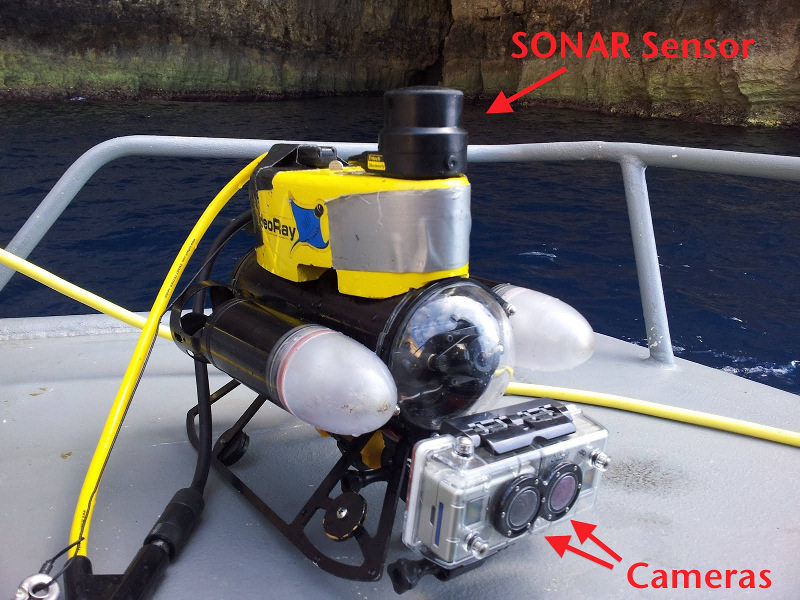
\epsfig{file = pics/ROV.jpg, width = 7cm}}
   \caption{Hardware setup, consisting of a Tritech SeaSprite sonar sensor and two vertically aligned HD GoPro cameras mounted on a VideoRay Pro III Micro ROV.}
  \label{fig:ROV}
 \end{figure}

While the ROV is navigating a cistern, two high-definition (HD) cameras mounted to the bow in a waterproof casing are triggered to synchronously capture images every second. The cameras are vertically aligned so as to minimize image disparity in the vertical direction. 
This environment and setup presents a number of challenges for disparity mapping.  
Most importantly, the ROV's thrusters disturb sediment and other small objects in the environment, which then bespeckles the captured images.
Simple, single pass disparity algorithms were unable to produce good disparity maps from these images.  Instead we chose a more complex, multi-pass algorithm, as is detailed below. 

\section{\uppercase{Gross sonar Model Reconstruction}}
\label{sec:reconstruction}

%Discuss sonar models/how they are generated in our situation. More focused on the robotics aspect, rather than the details of Jeff and Billy's projects.

\noindent In this section we provide a background detailing the approach to rough geometry model generation from sonar input. Zoe" might be best at this... I think we just want to summarize it very fast and without too much detail so that we have more room for the stereo stuff. I tried to summarize section~\ref{sec:data} briefly as well, but perhaps we can shorten it a bit if we need more room. Mention that we extrapolate the near-ground scan plane into 3D in most cases, rather than having true 3D maps.

\begin{figure*}[!ht]
   \vspace{-0.2cm}
   \centering{
      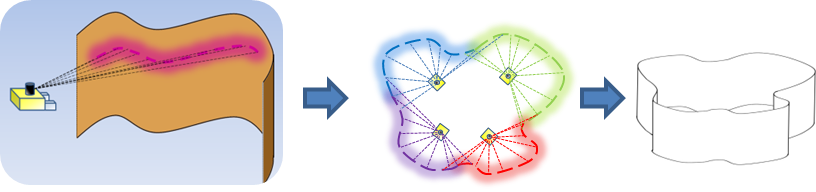
\epsfig{file = pics/1.png, width = 0.9\textwidth}}
   \caption{How we generate meshes from sonar models.}
  \label{fig:meshgen}
 \end{figure*}

\section{\uppercase{Fine Detail Additions Via Stereoscopic Depth Extraction}}
\label{sec:detail}

\noindent In this section we describe our approach towards the addition of fine details to the gross sonar models produced in Section~\ref{sec:reconstruction}. 

% Rough stub, delete/edit/use for inspiration!
The first step towards building fine details into a planar mesh is extracting those details. 
This is done by building disparity maps from the captured images.
The second step is taking those disparity and image pairs and using them to deform and texture, respectively, the basic sonar mesh. 

\noindent bla bla bla this produces a real-time 3D navigation interface for archaeologists to examine cisterns.

%Discuss why this is necessary. Discuss a system level overview of the process (more in depth than in introduction).

\subsection{Disparity Map Generation}

\begin{figure*}[!ht]
   \vspace{-0.2cm}
   \centering{
      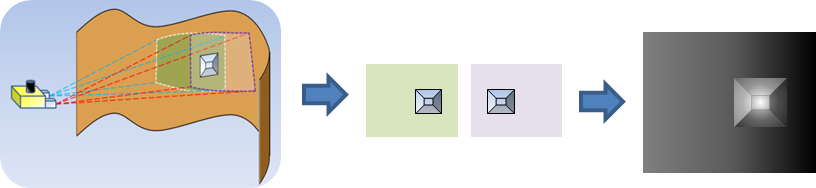
\epsfig{file = pics/2.png, width = 0.9\textwidth}}
   \caption{How we generate disparity maps from images.}
  \label{fig:dispgen}
 \end{figure*}


A number of algorithms currently exist to take two images, compare their features, and determine which points were closer and which were further from the camera (Figure~\ref{fig:dispgen}). 
Unfortunately, few of these algorithms were robust enough to handle compressed underwater images of rock walls.
We eventually chose the stereo mapping algorithm described by Zitnick and Kanade in "A Cooperative Algorithm for Stereo Matching and Occlusion Detection".

The main problem with our images is that we are dealing with a very dull landscape.  
Rocks, and especially bricks, have highly repetitive patterns and colors which produce feature-scarce images.
Most stereo-matching algorithms, including Zitnic and Kanade, rely on those features to determine disparity.  
The algorithm proposed by Zitnick and Kanade uses a scanning, sliding comparison window to build an initial disparity map.  
To mitigate the dull landscape, we choose a large initial disparity window with a radius of five. 
Obviously, this reduces the level of fine details that can be resolved from the image and adds a smoothing effect to the disparity map, but these drawbacks are acceptable in the given environment.  
Instead, a large window gives us a more reliable matching between rocks faces because it can encompass more features for each pixel.  

One of the strengths of the Zitnick and Kanade algorithm is its ability to detect occlusions.  
A common problem feature in our images is dirt particles, which are agitated by the ROV's positioning thrusters.
Usually the particles are small enough to be detected and removed from the final disparity map.

Another issue with underwater environments is lighting.
  Disparities in lighting between images, and as a result pixel intensities, is a common problem in our images.  
This is not handled by the Zitnick and Kanade algorithm and is discussed in greater depth in Section~\ref{subsec:hsl_color_correction}.


\subsubsection{Image Correction}
\label{subsec:image_correction}

In many stereo mapping algorithms, including Zitnick and Kanade, it is assumed that both images are accurate down to the pixel level.
Regrettably, the GoPro cameras that we used were limited to recording images in the lossy .jpeg format only.
To solve this issue we smoothed and shrunk the high resolution .jpeg images taken by the GoPros. 
This produced smaller left and right images that were comparable at the pixel level.

The smoothing step was performed to remove .jpeg artifacts.
  A simple Gaussian smooth was ineffective in this case because it blurred the edges of the rocks or bricks.
  Instead Photoshop's "surface smooth" was used to preserve edges while still blurring similar color regions.

The shrinking step was then performed on the image to further reduce the .jpeg artifacts and trim the size to something process-able.  
The best detail to process time ratio was obtained by reducing the images by one sixth.   
Shrinking was performed after smoothing to preserve the maximum amount of detail in the image.  


\subsubsection{Disparity Mapping}
\label{subsec:disparity_mapping}

Our disparity maps were generated using the cooperative, iterative approach described by Zitnick and Kanade (Include Reference).  
The basic algorithm is as follows:
\\ \\
1) Find the local support region for each pixel at (x,y) and each depth (d) by using an image intensity comparison function \(\delta\).  We chose \(\delta\) to be a normalized correlation function.
\[L_0(x,y,d) = \delta(I_{Left}(y,x),I_{Right}(y,x+d))\]
\\ \\
2) Copy the values from the 3D array \(L_0\) into a new 3D array \(L_n\).
\\ \\
3) Assume that, \(\Phi\)(x,y,d) is the 3D support region around the pixel (x,y), and suppose:
\[S_n(x,y,d) = \sum_{(x',y',d') \in \Phi} L_n (x+x', y+y', d+d') \]
Furthermore, assume that \(\Psi\)(x,y,d) is the set of all pixels that map to (x,y) in the left image and (x+d,y) in the right image. 
Let \(\alpha\) be a constant that controls how quickly the values in \(L_n\)(x,y,d) will converge.  
Then iterate through the values in \(L_n\) updating each value using: 
\[L_{n+1}(x,y,d) = \]
\[L_n(x,y,d)*\left(  \frac{S_n(x,y,d)}{\sum\limits_{(x'',y'',d'') \in \Psi(x,y,d)} S_n(x'',y'',d'')} \right)^\alpha \]
\\ \\
4) To build the final disparity map loop through each pixel position (x,y) and award the depth value (d) with the highest weight from \(L_n\)(x,y,d) as the final value.
If the best weight for all depths for a certain pixel (x,y) is below a predefined threshold, assume the pixel was occluded.

%\subsubsection{Post Disparity Generation Correction}
%\label{subsec:post_zitcan_correction}

%All of the disparity maps generated by the Zitnick and Kanade algorithm had slight errors around the edges.  
%Patches of the image would either be unreasonably close to the camera or flat against the background.  
%These images had to be corrected before they could be mapped to vertices.  

% possibly move to future works section?
\subsubsection{HSL Color Correction}
\label{subsec:hsl_color_correction}
Unfortunately, the paired GoPro cameras that we choose for data collection lacked the ability to sync exposure times.  
The cameras independntly calculated the correct exposure for their image only, which resulted in a lack of light intensity matching between left and right images.
A potential solution to this problem lies in using a color comparision function instead of an intensity comparison function (reference: "Stereo vision for robotic applications in the presence of non-ideal lighting conditions").
The solution proposed by Nalpandtidis and Gasteratos suggests converting the images into the HSL color space and looking at only the hue and saturation values.  
 
For our purposes, however, this method failed.  
Many of the surfaces that we imaged were gray in color producing uniform hue and saturation values.
For future experiments, introducing a light with a distinct color, perhaps blue, could prove useful for gray surfaces.  
This blue light would provide definate hue and saturation values that could be compared regardless of exposure times.


\subsubsection{Calibration}
\label{subsec:calibration}

An important step in any meaningful disparity mapping is calibration.
This is the creation of a tuned mapping from an (r,g,b) pixel value to the appropriate vertex offset in the virtual world. 
We were able to cheat slightly on this calibration because we were tuning for a very short field of view, 0.2m - 1.2m.
This allowed us to approximate a linear relationship between a disparity value and its physical depth. 

The images and values for the calibration were taken in a controlled pool environment.  
Pictures of a patterned surface were taken at a number of measured distances from that surface. 
Those images were then disparity mapped, and the average disparity at the center of the picture was used as the disparity data point for that physical depth.
Using this set of points we were able to create a linear mapping between disparity and depth.


\subsection{Projective Texturing}

%Describe how projective texturing works, describe how vertices are selected, describe phantom texture vs. displayed texture, then jump into math mode.

%Explains the method implemented to displace vertices. Discuss the use of a phantom texture to displace vertices, and the use of a photograph texture overlaid on the same wall segment. Discuss why displacing along toProjector is better than displacing along normal (graphic would be helpful). 

%Computation of plane eqs, acquire list of vertices contained within frustum, shader texturing. Explain why $\begin{Vmatrix}C\end{Vmatrix}$ is correct, talk about blending, explain how to determine whether vertex lies within frustum and how to texture map.

\noindent In order to add fine details to the gross sonar generated mesh, we use projective texturing. Rather than implementing (traditional? is there a better word?) texturing, projective texturing is utilized because of its ability to properly simulate an ROV as a point particle with the ROV's view frustum modeled as six implicit plane equations. This similarity enables a 'copy paste' method of texturing, where the ROV captures an image of an organic feature in a cistern, and a projector casts the image from the same relative position onto the a gross sonar reconstruction (Figures~\ref{fig:dispgen},~\ref{fig:projtex}). 

OpenGL and OpenGL Shading Language (GLSL) graphics libraries are utilized to aid in projective texturing, the latter being used to create shaders - small programs run per-vertex directly on the GPU. The shaders are programmed to selectively alter rendered vertex information, such as position (vertex shader) and color (fragment shader). The combination of projective texturing and stereoscopic imaging enables the ability to selectively displace vertices according to the color of a texture-mapped disparity map that is projected onto a surface. These vertices are displaced along the vector leading from their original 3D position in the mesh to the position of the projector, re-applying the geometry captured within the cistern to the model.

A projector is simulated by establishing plane equations for a view frustum based on the position and orientation of the ROV when the projected images were captured in a cistern. We define $J = \{j_{1},\dots,j_{N}\}$ to be the set of projectors casting textures onto the gross surface reconstruction. Each projector, $j_{n} = ((j_{n_{x}}^{pos},j_{n_{y}}^{pos},j_{n_{z}}^{pos}), \langle j_{n_{x}}^{look},j_{n_{y}}^{look},j_{n_{z}}^{look}\rangle)$, is uniquely defined by its position in 3D space, and a look vector orthonormal to the projector's viewport (Figure~\ref{fig:frustum}). All projectors have a pre-calibrated Field Of View (FOV) mimicking the compound FOV produced by the GoPro camera and waterproof housing lenses. The ROV is not equipped with roll thrusters, allowing us to ignore the possibility of a tilted camera frustum (i.e. the projector's right facing vector will always lie in the horizontal plane). Implicit plane equations modeling the projector view frustums in the form $Ax + By + Cz + D = 0$ are resolved using the approach in [CITATION NEEDED], where $\langle A, B, C\rangle$ is the plane's normal vector and  $(x, y, z)$ is a point on the plane. In this approach, plane equations are computed in homogenous space using the composite $4x4$ modelview projection matrix of the projector, $\lbrack \chi \rbrack$.

\begin{align}
\nonumber %Left plane
&\lbrack A \hspace{3pt} B \hspace{3pt} C \hspace{3pt} D \rbrack^\mathrm{T}_{Left} \hspace{-15pt} &= \hspace{10pt}&\lbrack \chi_{11} \cdots \chi_{41} \rbrack^\mathrm{T} + \lbrack \chi_{14} \cdots \chi_{44} \rbrack^\mathrm{T}
\\
\nonumber %Right plane
&\lbrack A \hspace{3pt} B \hspace{3pt} C \hspace{3pt} D \rbrack^\mathrm{T}_{Right} \hspace{-15pt} &= -&\lbrack \chi_{11} \cdots \chi_{41} \rbrack^\mathrm{T} + \lbrack \chi_{14} \cdots \chi_{44} \rbrack^\mathrm{T}
\\
\nonumber %Top plane
&\lbrack A \hspace{3pt} B \hspace{3pt} C \hspace{3pt} D \rbrack^\mathrm{T}_{Top} \hspace{-15pt} &= \hspace{10pt}&\lbrack \chi_{12} \cdots \chi_{42} \rbrack^\mathrm{T} + \lbrack \chi_{14} \cdots \chi_{44} \rbrack^\mathrm{T}
\\
\nonumber %Bottom plane
&\lbrack A \hspace{3pt} B \hspace{3pt} C \hspace{3pt} D \rbrack^\mathrm{T}_{Bot} \hspace{-15pt} &= -&\lbrack \chi_{12} \cdots \chi_{42} \rbrack^\mathrm{T} + \lbrack \chi_{14} \cdots \chi_{44} \rbrack^\mathrm{T}
\\
\nonumber %Near plane
&\lbrack A \hspace{3pt} B \hspace{3pt} C \hspace{3pt} D \rbrack^\mathrm{T}_{Near} \hspace{-15pt} &= \hspace{10pt}&\lbrack \chi_{13} \cdots \chi_{43} \rbrack^\mathrm{T} + \lbrack \chi_{14} \cdots \chi_{44} \rbrack^\mathrm{T}
\\
\nonumber %Far plane
&\lbrack A \hspace{3pt} B \hspace{3pt} C \hspace{3pt} D \rbrack^\mathrm{T}_{Far} \hspace{-15pt} &= -&\lbrack \chi_{13} \cdots \chi_{43} \rbrack^\mathrm{T} + \lbrack \chi_{14} \cdots \chi_{44} \rbrack^\mathrm{T}
\\
\end{align}

\begin{figure}[!h]
   \vspace{-0.2cm}
   \centering{
      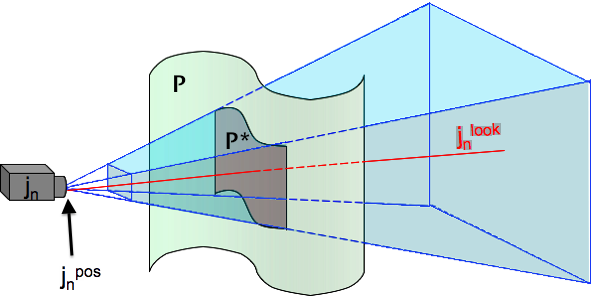
\epsfig{file = pics/frustum.png, width = 7cm}}
   \caption{Frustum and viewport.}
  \label{fig:frustum}
 \end{figure}

Next, for each projector, all faces in the mesh are passed through a view frustum culling filter in order to produce a list of faces contained within the frustum. We define $P = \{p_{1},\dots,p_{M}\}$ to be the set of vertices contributing to the gross sonar reconstructed mesh. Each vertex, $p_{n} =  (p_{m_{x}},p_{m_{y}},p_{m_{z}})$, is defined by its position in 3D space. Additionally, we define $F = \{f_{1},\dots,f_{Q}\}$ as the set of faces in the mesh. Each face, $f_{q} = (p_{\alpha}, p_{\beta}, p_{\gamma})$, is comprised of three vertices. We begin with a (un-memory-intensive... find another way to phrase - perhaps list big O notation?) preliminary cull which discards faces if their bounding sphere is outside of the projector's view frustum. Since frustum planes are modeled implicitly with normal vectors pointing into the frustum, if the signed distance from the face's center to the frustum plane, $\delta_{center}$, is less than the negative of the face's bounding sphere's radius, then the face's bounding sphere is entirely outside of the view frustum. In this case the face is immediately culled. $\delta_{center}$ is computed as follows,
%
\begin{equation}
\delta_{center} = \frac{Ax + By + Cz + D}{3 \begin{Vmatrix} \langle A, B, C \rangle \end{Vmatrix}},
\end{equation}

where
\begin{equation}
(x, y, z) = \left(\sum\limits_{\forall p_{m} \in f_{q}} p_{m_{x}}, \sum\limits_{\forall p_{m} \in f_{q}} p_{m_{y}}, \sum\limits_{\forall p_{m} \in f_{q}} p_{m_{z}}\right)
\end{equation}

Once faces are passed through the preliminary culling filter, a more memory-intensive (if you do list big O for prev cull, list it for this one too) thorough cull is executed in order to remove the small number of faces that lie entirely outside of the frustum, but whose bounding spheres are still intersected by the frustum plane.  To accomplish this, the signed distances from each vertex in the face to the frustum plane, $\delta_{\alpha}$, $\delta_{\beta}$, and $\delta_{\gamma}$, are individually computed. If $\delta_{\alpha}$, $\delta_{\beta}$, and $\delta_{\gamma}$ are all less than zero, the face is culled. $\delta_{\alpha}$, $\delta_{\beta}$, and $\delta_{\gamma}$ are computed as follows,
%
\begin{equation} % fix this... shitty eqn
\delta_{\alpha, \beta, \gamma} = \frac{Ax + By + Cz + D}{\begin{Vmatrix} \langle A, B, C \rangle \end{Vmatrix}},
\end{equation}

where
\begin{align}
\nonumber
(x, y, z)_{\alpha} &= (p_{\alpha_{x}}, p_{\alpha_{y}}, p_{\alpha_{z}})\\
\nonumber
(x, y, z)_{\beta} &= (p_{\beta_{x}}, p_{\beta_{y}}, p_{\beta_{z}})\\
(x, y, z)_{\gamma} &= (p_{\gamma_{x}}, p_{\gamma_{y}}, p_{\gamma_{z}})
\end{align}


With faces lying outside of the projector view frustums culled, the vertices in the remaining faces are added to a trimmed set, $P^{*}\subset P$, whose members are sent to the vertex and fragment shaders (i.e. to the GPU) to be and displaced and textured in accordance with the generated disparity map and camera image, respectively (Figure~\ref{fig:frustum}). $P$ is also sent to the GPU so that the portions of the mesh that are not displaced or textured are still rendered.

The implemented projective texturing method naturally produces a second projection facing in the direction negative to $j_{n}^{look}$. To remove the unwanted projections, a simple check was added to the vertex shader which ensures that the texture mapped vertex position has a positive $q$ component.

\subsection{Per-Vertex Computations}

A GLSL vertex and fragment shader are used to displace and texture vertices. The vertex shader recieves $P$ and $P^{*}$, as well as a modelview projection matrix for the camera and each projector, projector positions, texture primitives for the disparity maps, an offset and scale value for displacement magnitudes, and normal vectors used for lighting computations from the OpenGL program. The vertex shader displaces vertices one at a time in accordance with the color of the texture-mapped disparity map coordinates. Vertices vertices (those belonging to $P^{*}$ are updated and sent to the fragment shader for diffuse shading computations.

The fragment shader recieves $P$ and $P^{*}$, as well as the camera image texture primitives and the revised normal vectors of the vertices in $P^{*}$. The fragment shader maps the camera images onto the vertices in the frustum of each projector. Again, vertices lying in the frustum of two or more projectors have their colors blended. Once an RGB color value has been computed for the vertex, diffuse shading is added to the model.

\subsubsection{Vertex Displacement}

Vertices belonging to $P^{*}$ are displaced along the vector $\vec{b} = j_{n} - p_{m}$ a distance proportional to the magnitude of the RGB color value, $C = \langle C_{r}, C_{b}, C_{g} \rangle$, of the disparity map at the corresponding texture-mapped coordinates, $t_m$. Since the modelview projection matrix of each projector is accessible from the vertex shader, the texture-mapped coordinates of $p_m$, and thus, $C$ can be calculated per-vertex.

\begin{align}
t_{m} &= p_{m}\lbrack MVP \rbrack _{j_{n}} \\
C &= \langle t_{m\_red}, t_{m\_blue}, t_{m\_green} \rangle
\end{align}

Vertex displacement then proceeds as follows:

\begin{equation}
p_{m}' = \left \{ 
\begin{array}{ll}
p_{m} + \vec{b} (\begin{Vmatrix}C\end{Vmatrix} S + O) & \text{if} \quad p_{m} \in P^{*}\\
p_{m} & \text{otherwise}
\end{array},\right.
\label{eq:displace}
\end{equation}

where $p_{m}'$ is the displaced vertex position and $S$ and $O$ are a scale and offset factor. $S$ grants the ability to fit a function to the displacement distance.$O$ is generally negative, ensuring that vertices belonging to $P^{*}$ are both pushed and pulled from the model surface. In the current version of the software, both $S$ and $O$ are user-controlled. However, the world space coordinates of the sonar mesh are computed such that one unit in world space is equal to one meter in the cistern, so a true value for $S$ and $O$ can be calculated through calibration.
 
 \subsubsection{Blending}
 ...
 
 \subsubsection{Lighting}
 ...

\section{\uppercase{Results}}
\label{sec:results}

\subsection{Stereo Results}

The Zitnick and Kanade algorithm was shown to perform well against the Univerisity of Tsukuba's Multiview Image Database.  
In our tests, it performed similarly well with rocky underwater cystern images.  
One such output image is show in Figure~\ref{fig:disparity}.
This image was generated using an initial support region of size (11, 11, 5), and then an iterative local support region of size (13,13,5).
Note that this image has lighting differences between left and right image.

\begin{figure}[!h]
	\centering
		\subfigure[Left camera image]{\label{left}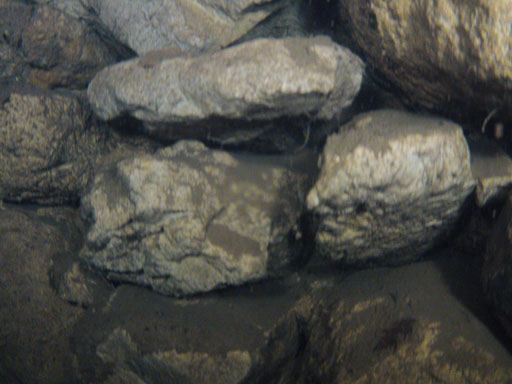
\epsfig{file = pics/372L.jpg, width = 3cm}}
		\quad %space between images
		\subfigure[Right camera image]{\label{right}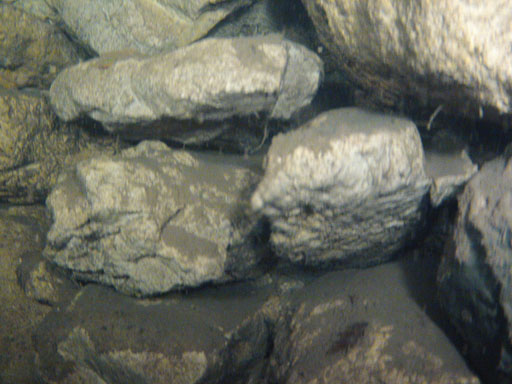
\epsfig{file = pics/372R.jpg, width = 3cm}}\\%new line
		\medskip
		\subfigure[Generated Disparity]{\label{disparitymap}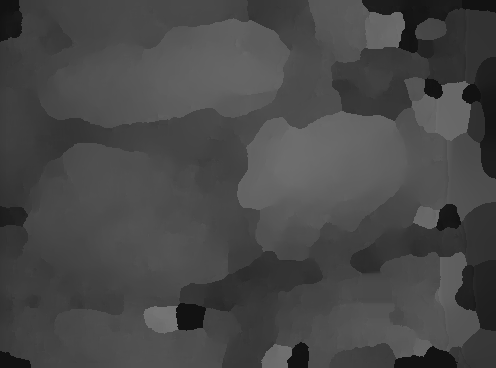
\epsfig{file = pics/372disp.png, width = 5cm}}
		\caption{Disparity Map generated with initial local support (13,13,5), and an iterative support of (11,11,5)}
		\label{fig:disparity}
\end{figure}

\subsection{Projection Results}
To demonstrate our complete stereo mapping system we deployed our VideoRay robot in a rock-walled well.
This well provided both a large simple cylindrical structure and a detailed bumpy surface.  

Using the Sonar data from the well we built the 3D figure shown in Figure~\ref{fig:result1}. 

\begin{figure}[!h]
	\centering
		\subfigure[Well Top View]{\label{left}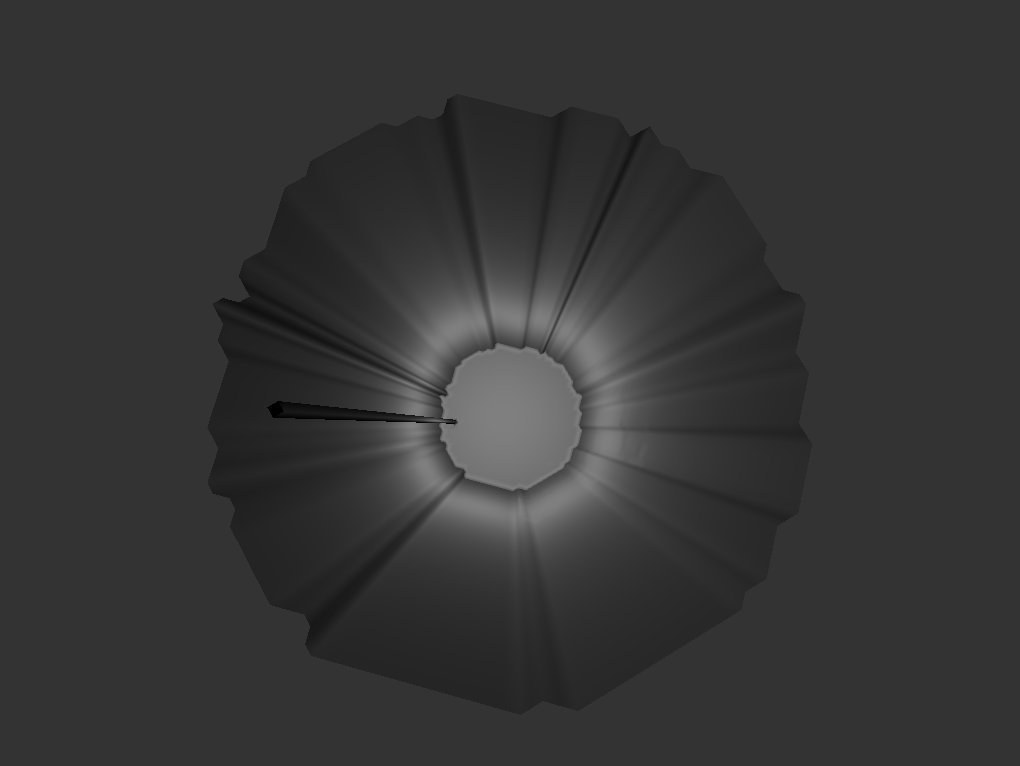
\epsfig{file = pics/blankWell1.png, width = 3.5cm}}
		\quad %space between images
		\subfigure[Well Side View]{\label{right}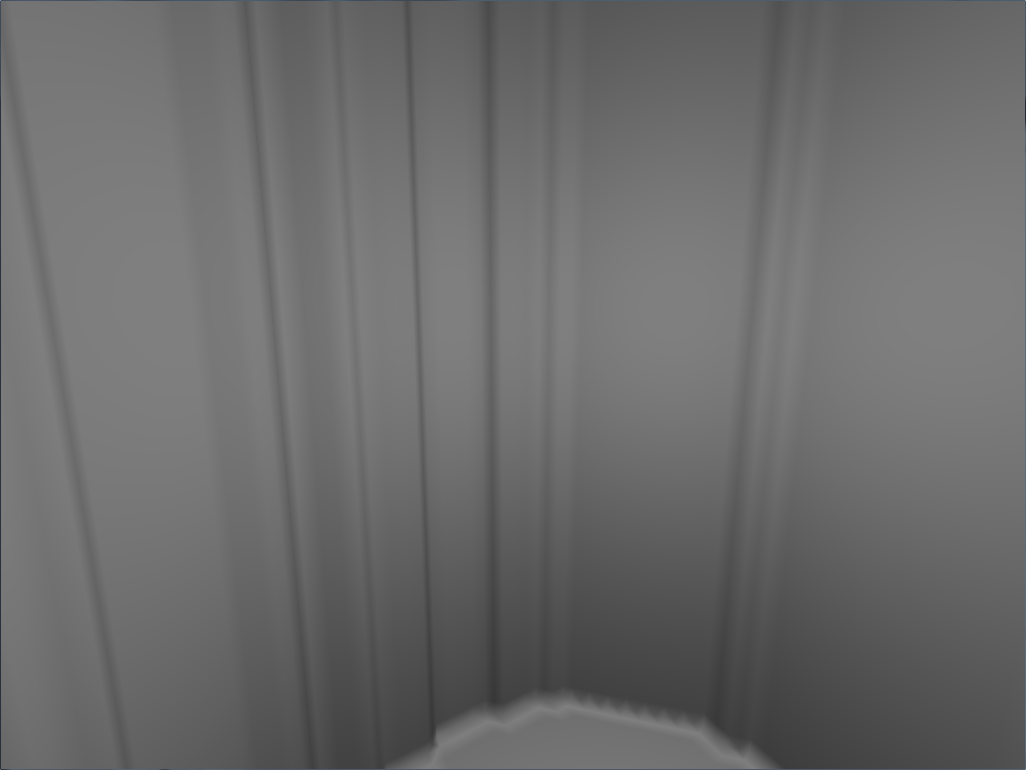
\epsfig{file = pics/blankWell2.png, width = 3.5cm}}\\%new line
		\caption{Views of Plain Well Geometry}
		\label{fig:result1}
\end{figure}

Inside that geometry we used virtual point projectors to display the rock textures that were taken at those locations (Figure~\ref{fig:result2}).

\begin{figure}[!h]
	\centering
		\subfigure[Projected Images]{\label{left}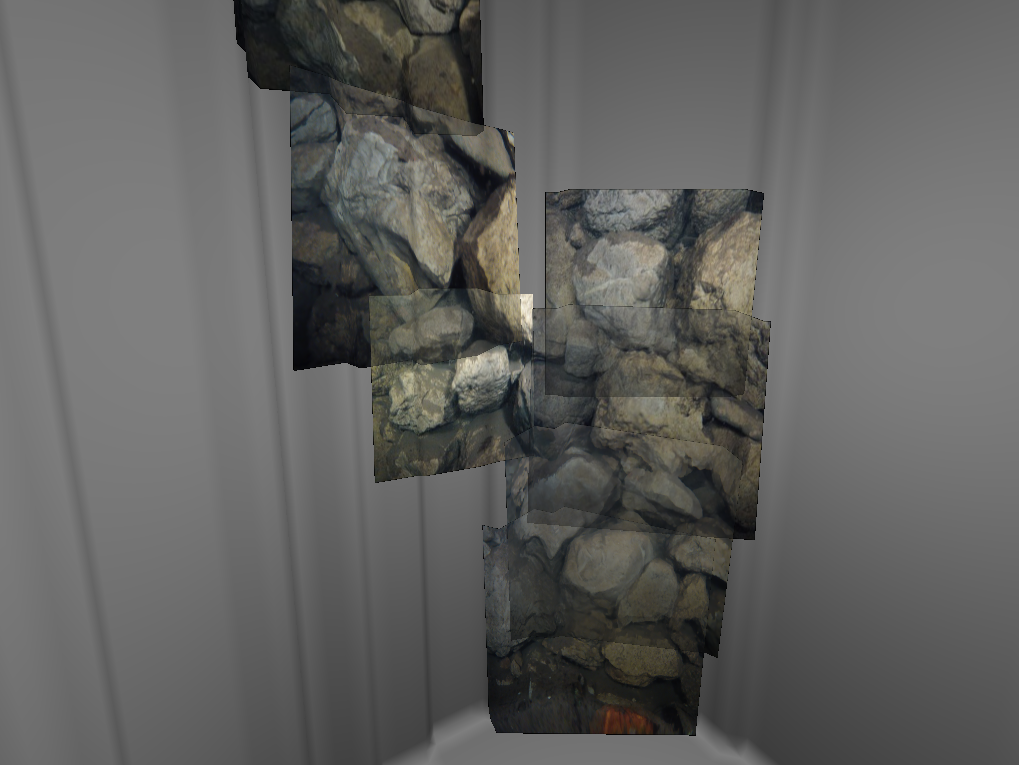
\epsfig{file = pics/noDisparity.png, width = 3.5cm}}
		\quad %space between images
		\subfigure[Images on Wireframe]{\label{right}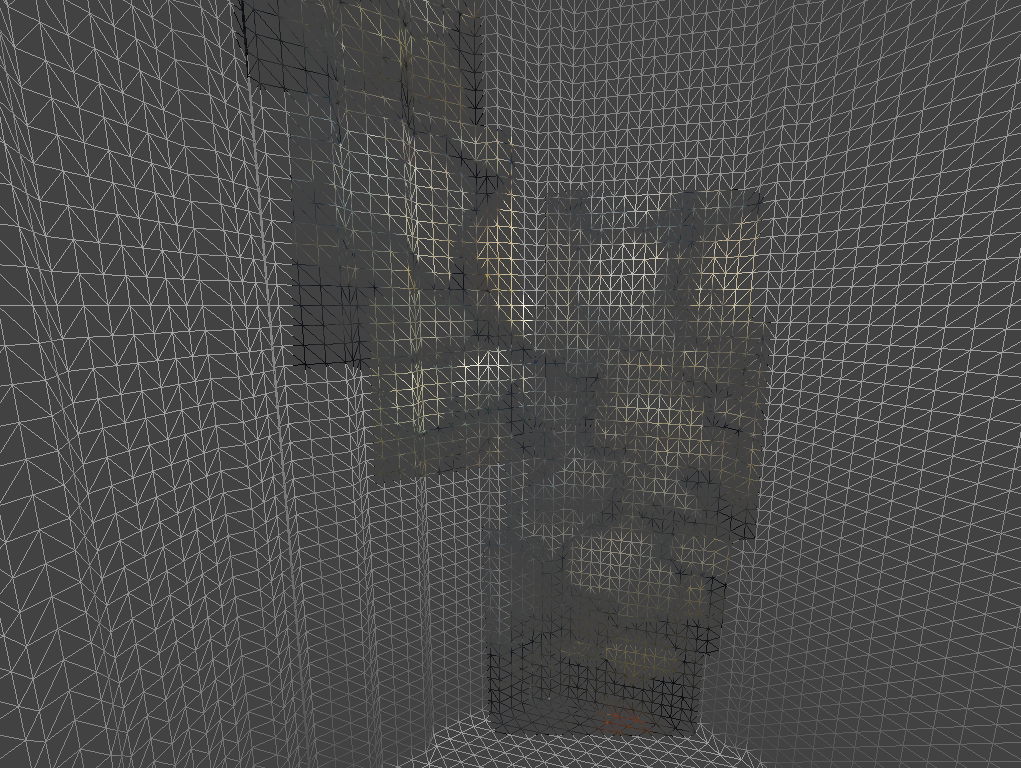
\epsfig{file = pics/noDisparityWire.png, width = 3.5cm}}\\%new line
		\caption{Well With Rock Textures}
		\label{fig:result2}
\end{figure}

  The disparity maps calculated at each of those points were then applied to deform the well geometry (Figure ~\ref{fig:result3}).

\begin{figure}[!h]
	\centering
		\subfigure[Projected Disparity Maps]{\label{left}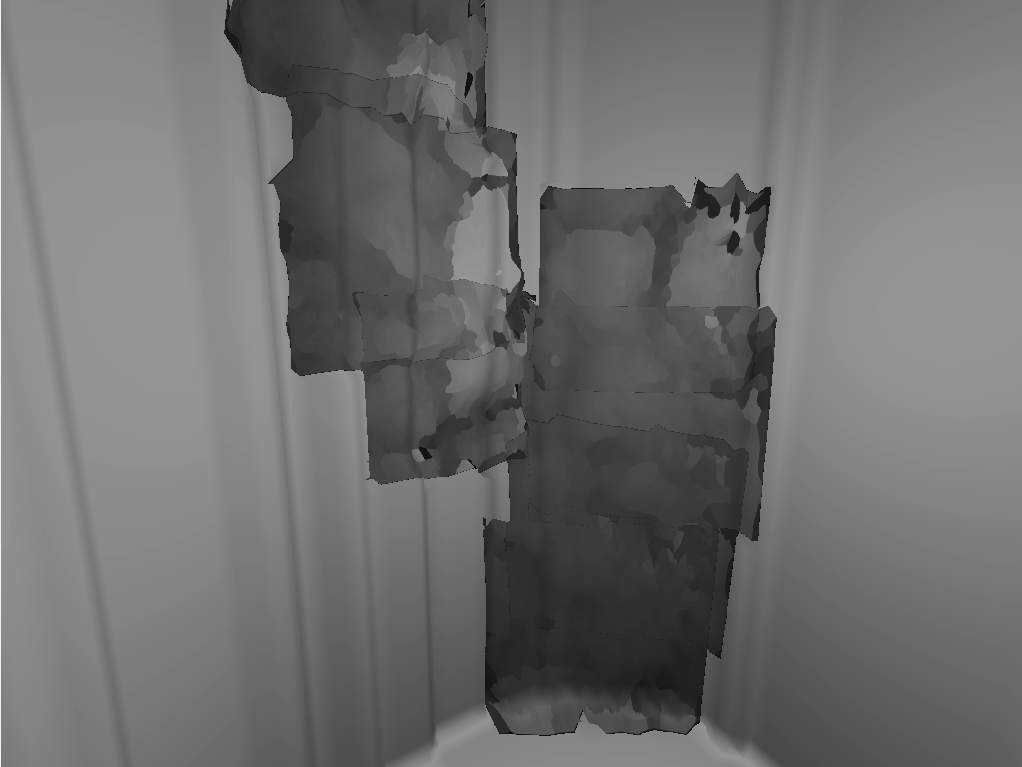
\epsfig{file = pics/mapsDisparity.png, width = 3.5cm}}
		\quad %space between images
		\subfigure[Wireframe Disparity Maps]{\label{right}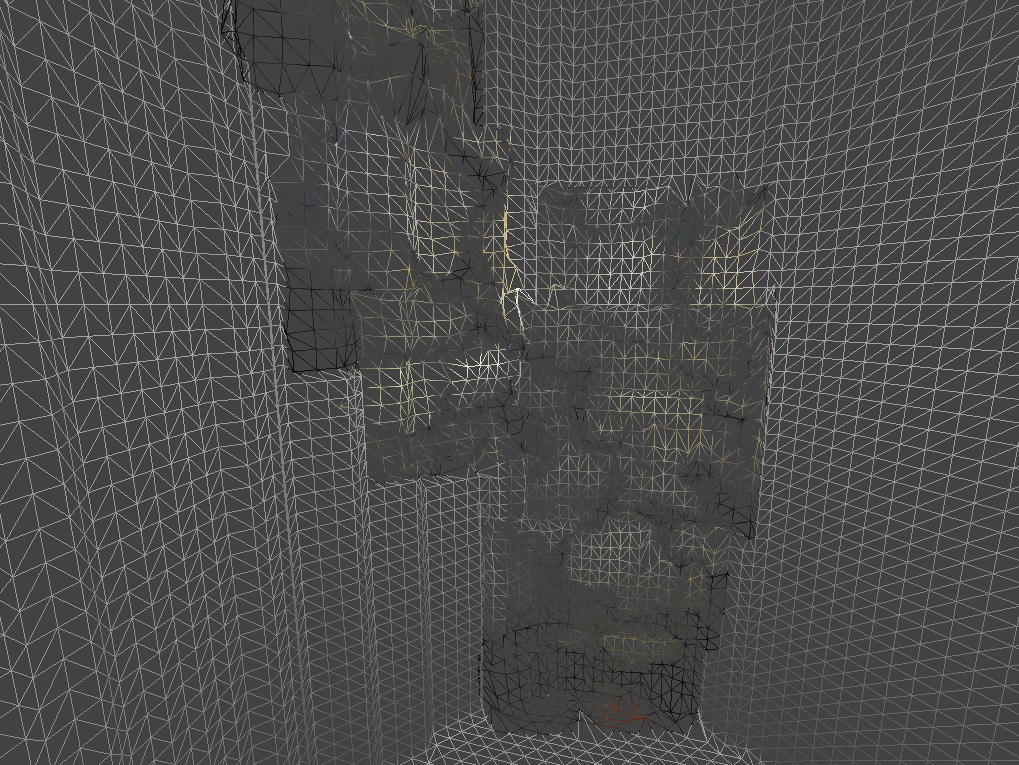
\epsfig{file = pics/disparityWire.png, width = 3.5cm}}\\%new line
		\caption{Well Deformed by Disparity Maps}
		\label{fig:result3}
\end{figure}

Finally, the disparity maps combined with the images were mapped into the well geometry to produce the final detailed mesh (Figures~\ref{fig:result4},~\ref{fig:resultFull}).  The only factor that is keeping us from filling the well with textures is the Glew texture limit. 

\begin{figure}[!h]
	\centering
		\subfigure[Well Wide Shot]{\label{left}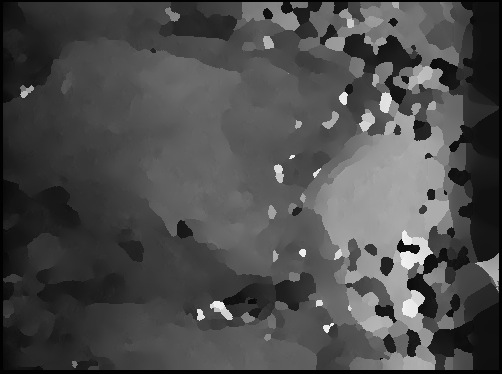
\epsfig{file = pics/disparity.png, width = 3.5cm}}
		\quad %space between images
		\subfigure[Rocks Closeup]{\label{right}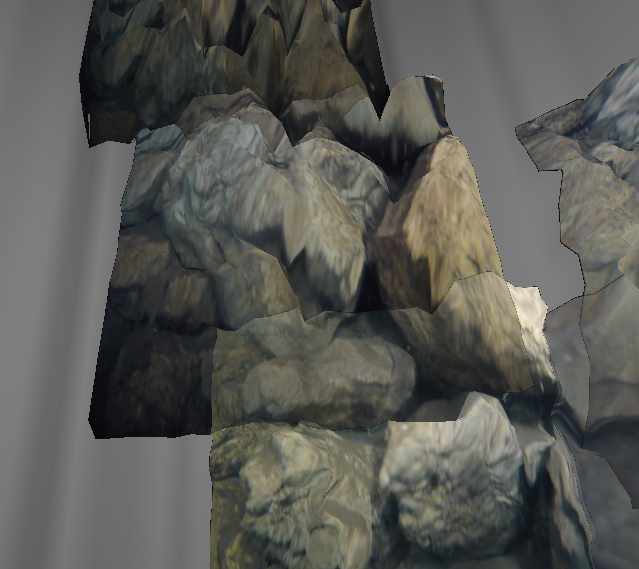
\epsfig{file = pics/mappedWell1.png, width = 3.5cm}}\\%new line
		\medskip
		\subfigure[Rocks Closeup Wireframe]{\label{center}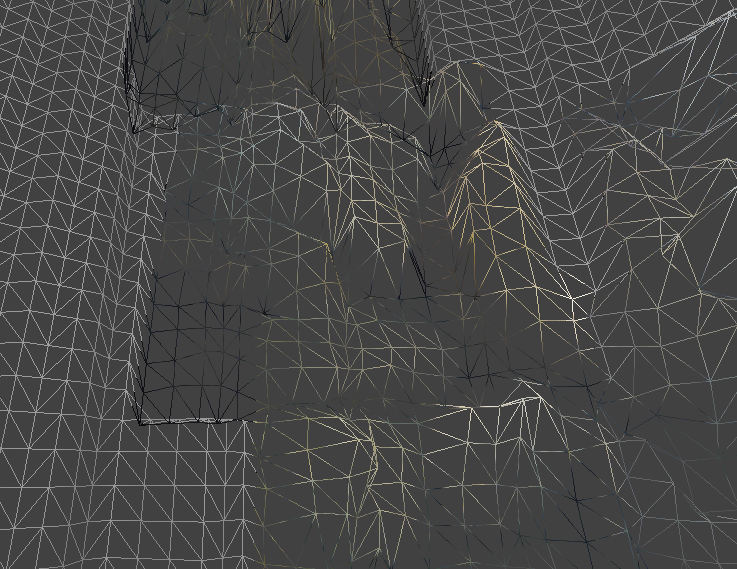
\epsfig{file = pics/mappedWell2.png, width = 6cm}}
		\caption{Fully Mapped Well}
		\label{fig:result4}
\end{figure}

\begin{figure*}[!ht]
   \vspace{-0.2cm}
   \centering{
      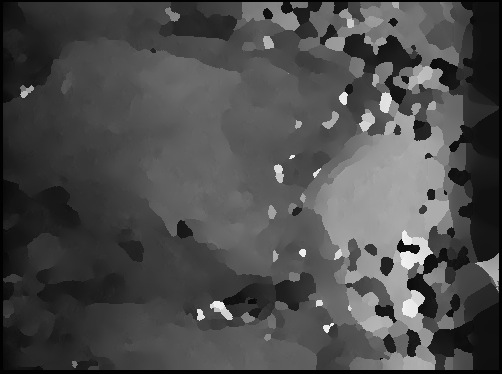
\epsfig{file = pics/disparity.png, width = .9\textwidth}}
   \caption{Full Displaced Well}
  \label{fig:resultFull}
 \end{figure*}

%\begin{figure*}[!ht]
%   \vspace{-0.2cm}
%   \centering{
%      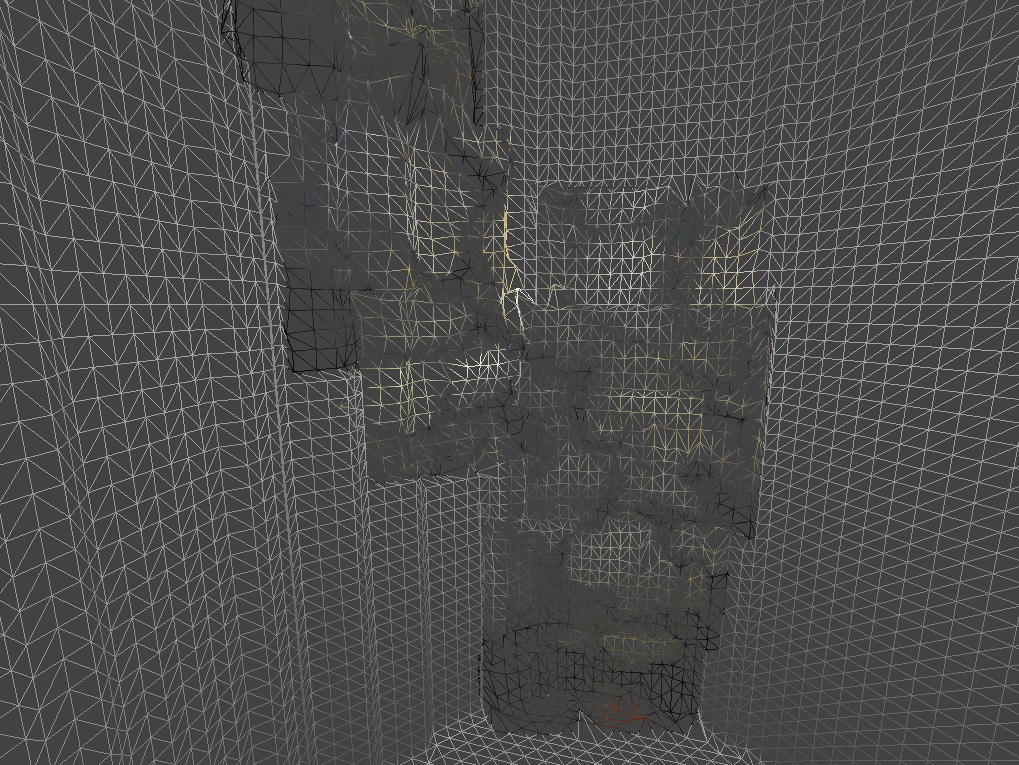
\epsfig{file = pics/disparityWire.png, width = .9\textwidth}}
%   \caption{Full Displaced Well, Wireframe}
%  \label{fig:resultFullWire}
% \end{figure*}

\section{\uppercase{Conclusion and Future Work}}
\label{sec:conclusion}

\noindent 
This paper presented a novel way to recreate detailed underwater environments.
It is motivated by the desire to better map underwater caverns and cisterns using robotic tools.  
In future experiments there are a few things that could be done to obtain better results.
The creation of more detailed disparity maps could be achieved by upgrading the cameras and the lights on the robot.  
GoPro cameras were a simple, cost-effective, solution to acquire underwater stereo images.  
The quality of those images, however, could be greatly increased with more professional hardware.  
With better cameras the output images would not need to be processed down to remove jpeg compression artifacts, which would allow much larger disparity images.  
Similarly, with better cameras there would be no need to compensate for different exposure times between images.
Alternatively, better lighting, including blue lighting, would allow pixel values to be compared in the HSL color space.  
Such hardware would reduce the need for a different camera setup.

In the future it would be interesting to explore the possibility of integrating this algorithm with a SLAM algorithm and more computing power to allow a robot to autonomously image each surface of a cistern. 
Unfortunately, that would require a far more complex setup that what we had available at the time of writing.

\bibliographystyle{apalike}

\bibliography{Stereo}

\end{document}

